

\subsection{Pulsweitenmodulation und ihre Darstellung}
\label{sec:PWM_Grundlagen}
Pulsweitenmodulation (PWM) ist eine Schlüsseltechnik in DC-DC-Wandlern, die zur Steuerung der Schaltkomponenten eingesetzt wird, um die Ausgangsspannung oder den Ausgangsstrom zu regulieren. Sie ermöglicht eine präzise Kontrolle, indem sie die 'Einschaltzeit' des Schalters im Vergleich zur gesamten Zykluszeit (Einschaltzeit + Ausschaltzeit) variiert.\cite{peddapelli2017pulse}

\paragraph{Tastverhältnis \(D\)}
Die Einschaltzeit ist die Zeit, der Schalter eingeschaltet ist. Das Tastverhältnis \( D \) wird mathematisch als das Verhältnis der Einschaltzeit zur gesamten Zykluszeit beschrieben:
\begin{equation}
D = \frac{\text{Einschaltzeit}}{\text{Einschaltzeit} + \text{Ausschaltzeit}}
\end{equation}

\paragraph{Proportionalanteil (P)}
Das Tastverhältnis spielt eine wichtige Rolle, da es den Mittelwert der Ausgangsspannung oder des Ausgangsstroms bestimmt. Bei der PWM wird ein Steuersignal mit einem hochfrequenten Trägersignal verglichen, um die 'Ein'- und 'Aus'-Zustände des Schalters festzulegen. Das Steuersignal stammt oft von höheren Regelkreisen wie PID-Reglern, die den Fehler zwischen Soll- und Istwert minimieren sollen.

Die Hauptmotivation für die Verwendung von PWM in Steuerungssystemen ist die Anpassung des Mittelwerts der Ausgabe an ein Referenzsignal. Zusätzlich wird versucht, harmonische Verzerrungen und Schaltverluste zu minimieren \cite{peddapelli2017pulse}.

In der Abbildung \ref{fig:PWM_converter} ist eine typische PWM-Schaltung dargestellt. Der PWM-Block und die Spannungsrückführungsschaltung im DC-DC-Wandler arbeiten zusammen, um sicherzustellen, dass die Ausgangsspannung der Referenzspannung folgt. Hierbei wird ein Steuersignal \(v_{\text{con}}\) und ein Rampensignal \(V_{\text{ramp}}\) verwendet, um die Impulsbreite des aktiven Schalters zu modulieren. Das rechte Diagramm (b) zeigt die Steuersignale und ihre Relation zueinander, wodurch das Schaltverhalten des Wandlers beeinflusst wird \cite{choi2013pulsewidth}.



\begin{figure}[htbp]
    \centering
    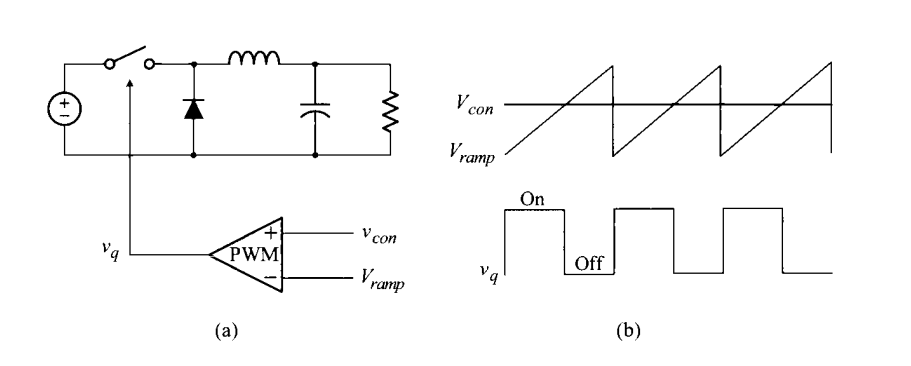
\includegraphics[width=0.8\linewidth]{2Grundlagen/141PWM.png}
    \caption{Schematische Darstellung eines PWM-Modulator. Quelle: \cite{choi2013pulsewidth}}
    \label{fig:PWM_converter}
\end{figure}
